% Talk.tex

%%%%
%  %
%%%%
\documentclass{beamer}
%%%%
%  %
%%%%

\usepackage[T1]{fontenc}
\usepackage{ucs}
\usepackage[utf8x]{inputenc}
%\usepackage[frenchb]{babel}
\usepackage{amsmath}
\usepackage{amssymb}
\usepackage{latexsym}
\usepackage{verbatim}
%\usepackage{moreverb}
\usepackage{fancyvrb}
%\usepackage{alltt}
\usepackage{eurosym}

\usepackage{hyperref}
\usepackage{colortbl}
%%%\usepackage{xlop}

%\usepackage{beamerthemesplit}
%\usetheme{Warsaw}
\useinnertheme[shadow=true]{rounded}
\usecolortheme{orchid}
\usecolortheme{whale}
\useoutertheme{shadow}

%\usepackage{beamerthemetree}

%\usepackage{epsfig}
\usepackage{graphicx}
\usepackage{pgf}
%\usepackage{pgf,pgfarrows,pgfshade}

\newcommand{\thepath}{.}

\newcommand{\imgpath}{\thepath/images}
\newcommand{\pdfteximgpath}{\thepath/pdftex}
\newcommand{\pdftextimgpath}{\thepath/pdftex_t}

\newcommand{\BBZN}{$0\nu\beta\beta$}
\newcommand{\BBZNM}{$0\nu\beta\beta\chi$}
\newcommand{\BB}{$\beta\beta$}
\newcommand{\BBDN}{$2\nu\beta\beta$}

\pgfdeclareimage[width=1.5cm]{logo}{\imgpath/snemo_snail_1.pdf}

%%%%%%%%%%%%%%%%%%%%%%%%%%%%%%%%%%%%%%%%%%%%%%%%%%%%%%%%%%%%%%%%%%%%%%%%%%%%%%%

\title[The SNRS package]{The SNRS package for realistic modelling of SuperNEMO source foils\\(updated 2021-05-29)}

\author[\tiny F.Mauger]{\small F.Mauger (LPC Caen, UNICAEN)}
\date[May, 2021]{\small SuperNEMO Collaboration Meeting, remote, May 10-12, 2021}

%%%%%%%%%%%%%%%%%%%%%%%%%%%%%%%%%%%%%%%%%%%%%%%%%%%%%%%%%%%%%%%%%%%%%%%%%%%%%%%

\logo{\pgfuseimage{logo}}

\begin{document}

\frame{
  \titlepage
}

\normalsize

%%%%%%%%%%%%%%%%%%%%%%%%%%%%%%%%%%%%%%%%%%%%%%%%%%%%%%%%%%%%%%%
\frame{

  \footnotesize

  \frametitle{What we have...}

  \only<1>{

    \begin{block}{The odd geometry of SuperNEMO source strips}

      \begin{itemize}
      \item Installation of source foils in september 2018 (A.Jeremie et al., DocDB-4705)
      \item Two layouts: ITEP style (long single strips) and LAPP style (vertical assembly of 8 pads)
      \item But important mechanical strain on materials:
        \begin{itemize}
        \item ITEP-style strips are deformed with rather large amplitude (several centimeters)
        \item LAPP-style strips/pads are also deformed ($o$(1 cm))
        \end{itemize}
      \item Optimization of the positioning of each strip,
        some mounting adaptation for very deformed strips (see Andrea's slides above)
      \end{itemize}

    \end{block}

  }

  \only<2>{

    \begin{block}{3D-measurement of the source foils geometry}

      \begin{itemize}
        
      \item 3D tracker measurements (nov. 2019, see report and first analysis by Y.Lemière, DocDB 4954)

      \item Originally done to measure the positioning of the tracker structure and cells

      \item Also available: a snapshot of deployed calibration sources and source foils

      \item Raw \textit{Laser Tracker Data} (LTD) dataset, available package at CCIN2P3:

        \texttt{/sps/nemo/snemo/snemo\_data/misc/SNLTD\_3D\_measurements-1.0.tar.gz}
        
      \end{itemize}

    \end{block}

  }

  \only<3>{
    Full Y-Z view of the source frame with 3D laser measurements (from Italian side):
    \begin{center}
      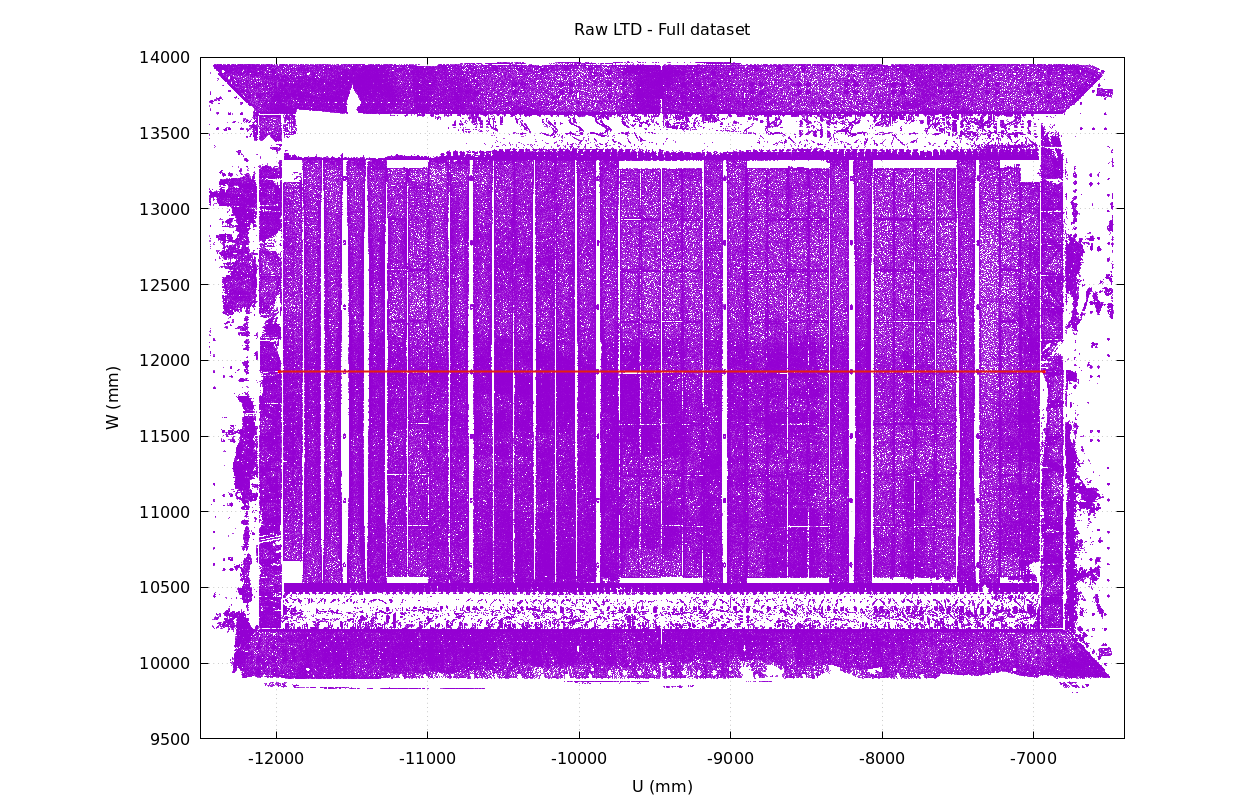
\includegraphics[width=\linewidth]{images/raw_ltd_source_foils_1.png}
    \end{center}
  }
  
  \only<4>{
    Top X-Y view with positions of cathode rings and source foils:
    \begin{center}
      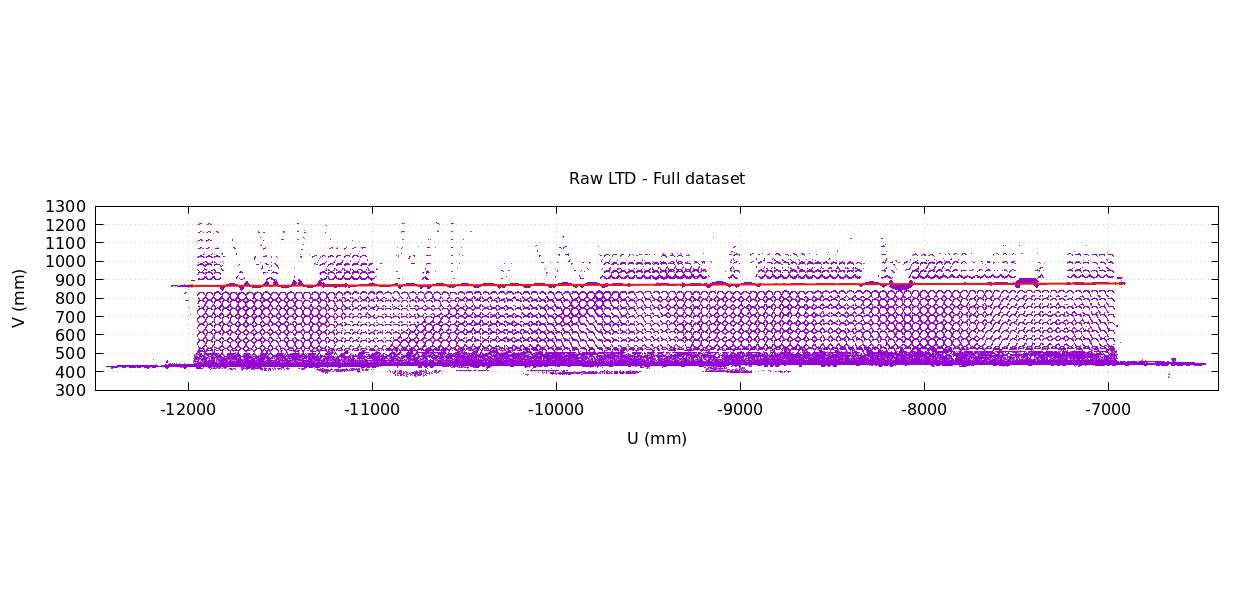
\includegraphics[width=\linewidth]{images/raw_ltd_source_foils_2.png}
    \end{center}
  }
  
  \only<5>{
    Top view of block 0 (mountain side, source strips 0 to 2):
    \begin{center}
      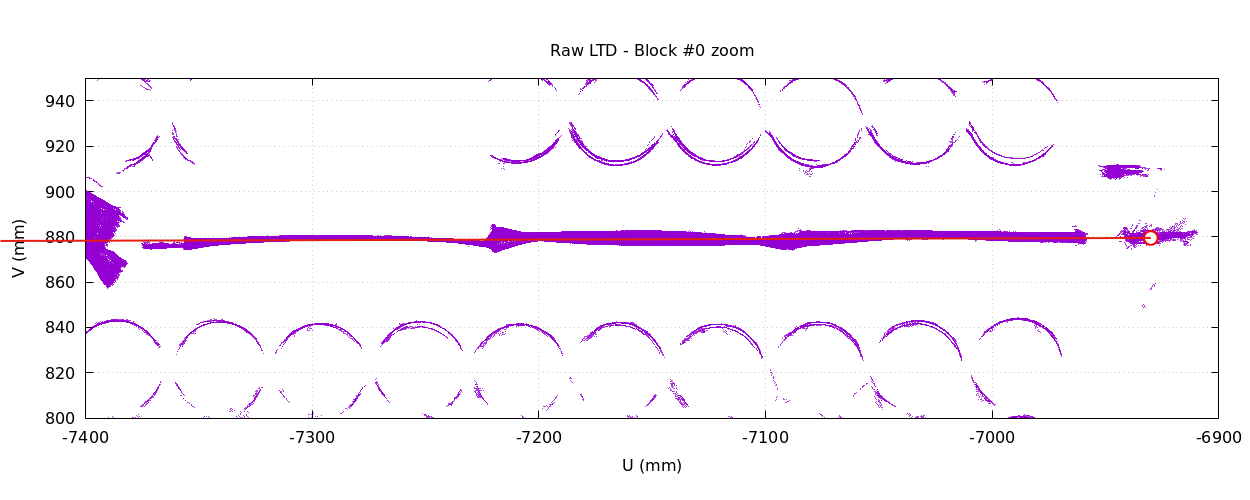
\includegraphics[width=\linewidth]{images/raw_ltd_source_foils_3.png}
    \end{center}
    Small deformations of the strips (alternate curvatures) at a few millimeter scale (LAPP style and copper foil)
  }
  
  \only<6>{
    Top view of block 6 (tunnel side, source strips 33 to 35):
    \begin{center}
      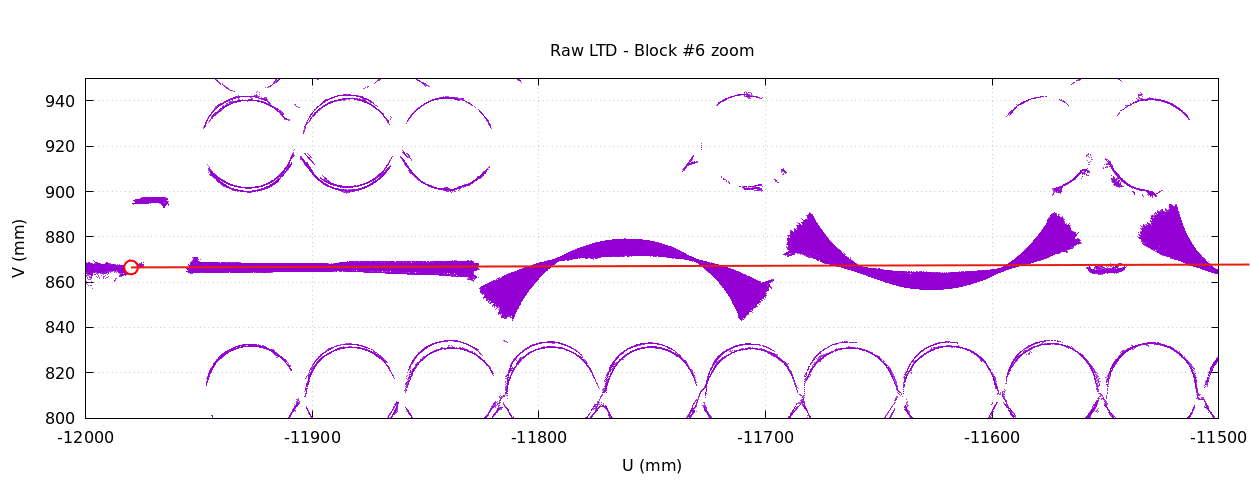
\includegraphics[width=\linewidth]{images/raw_ltd_source_foils_4.png}
    \end{center}
    Large deformations of the strips at a few centimeter scale (ITEP style)
  }
  
  \only<7>{
    Top view of block 3 (central source strips): \\
    \begin{center}
      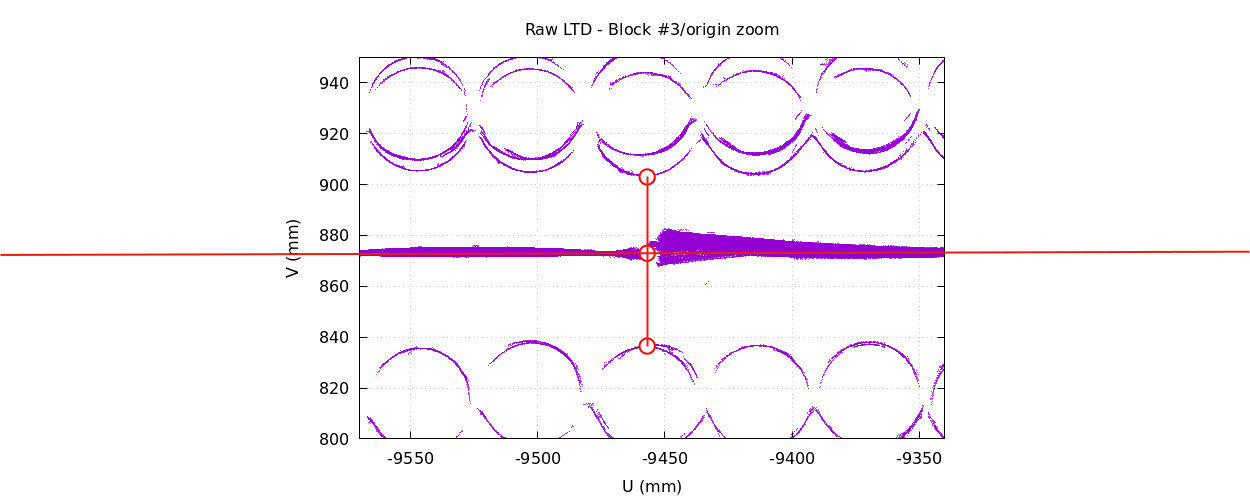
\includegraphics[width=\linewidth]{images/raw_ltd_source_foils_5.png}
    \end{center}
    Reconstruction of the origin of the SuperNEMO demonstrator frame.
    \vskip 5pt
    Also, misalignement of bottom and top cathode rings.
  }
 

  \only<8>{

    \begin{block}{Objective of this study: using raw LTD data for a better understanding and modelling
      of the geometry of source foils}

      \begin{itemize}
        
      \item Extraction of raw LTD datasets per source blocks (preliminary work done by Y.Lemière, 2019)

      \item Description in DocDB-5400 (F.Mauger) with calibration of positions/orientation

      \item Conclusion, laser measurements at submillimetric precision, $\simeq$500 $\mu$m along X,Y,Z axis

      \item Should be enough to build a precise geometry model for simulation
        and the reconstruction/analysis software.
  
        
      \end{itemize}

    \end{block}

  }
 

  \only<9>{

    \begin{block}{Conclusion of this first stage work}

      \begin{itemize}
 
      \item Source deformation of ITEP style foils at centimeter scale :

        $\leadsto$ this is at the level of the expected
        resolution for vertex reconstruction.

      \item Preliminary intuition: it is needed to work with a realistic model of this deformed geometry

      \item Current implementation of the source foils in the Falaise software (Y.Lemière, F.Mauger) :
        $\leadsto$ flat realistic models for source foils with ITEP/LAPP style

        \begin{itemize}

        \item maybe enough for LAPP (8 pads) foils (small deformation),

        \item but ITEP foils are badly modelled considering the real situation    
        
        \end{itemize}

        
      \end{itemize}

    \end{block}

  }
   
}

%%%%%%%%%%%%%%%%%%%%%%%%%%%%%%%%%%%%%%%%%%%%%%%%%%%%%%%%%%%%%%%
\frame{

  \footnotesize

  \frametitle{The SNRS software package}

  \only<1>{

    \begin{block}{Objectives}

      \begin{itemize}
        
      \item Use the raw LTD datasets on a per source strip basis in order to build a realistic model
        of ITEP style foils.
        
      \item Step 1 : build calibrated LTD dataset per foil in the working reference frame of SuperNEMO (Falaise)

      \item Step 2 : use the former datasets to fit the shape of the source foils with a reasonnably simple curve (elliptic fit\dots)

      \item Step 3 : build a 3D-mesh geometry model of each source strip from the above fit (including
        the Se source pad and surrounding Mylar films %% (tessellated data)

      \item Step 4 : implement an efficient vertex generator to generate decay vertexes in the bulk/surfaces of the foils.

      \item Put everything in a single software package, comptible with Bayeux and Falaise : SNRS, \textit{SuperNEMO Realistic Source(s)}

      \item Step 5 : adapt reconstruction code in Falaise (on-foil vertex extrapolation on tracks).
        
      \end{itemize}

    \end{block}

  }

  \only<2>{

    \begin{block}{Step 1 : build LTD datasets}

      
      \begin{itemize}
        
      \item Described in DocDB \#5425
       
      \item Software tools to:

        \begin{itemize}
  
        \item extract per source foil calibrated LTD datasets
          
        \item sample Z-bands of 3D laser measurement points as input for a further fit

        \end{itemize}
  
        
      \end{itemize}

    \end{block}
  }

  \only<3>{

    %\begin{exampleblock}{
    Calibrated LTD datasets:
    \vskip 2pt

      Full dataset and highlighted Z-band of \textit{laser} 3D points (typical width: 1 mm)
      \begin{center}
        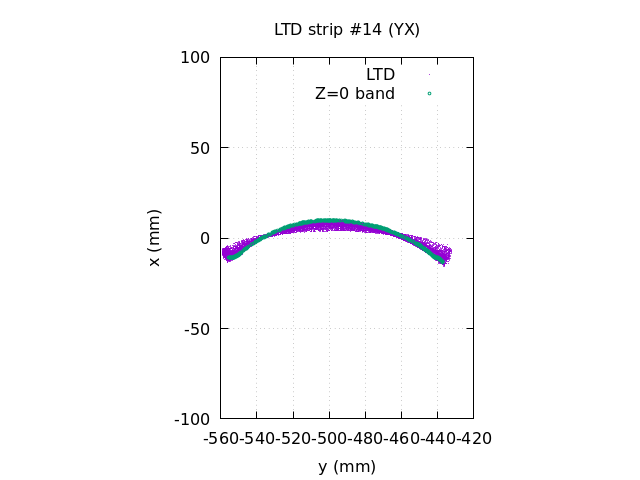
\includegraphics[width=0.45\linewidth]{images/snrs-ltd-strip14-1.png}
        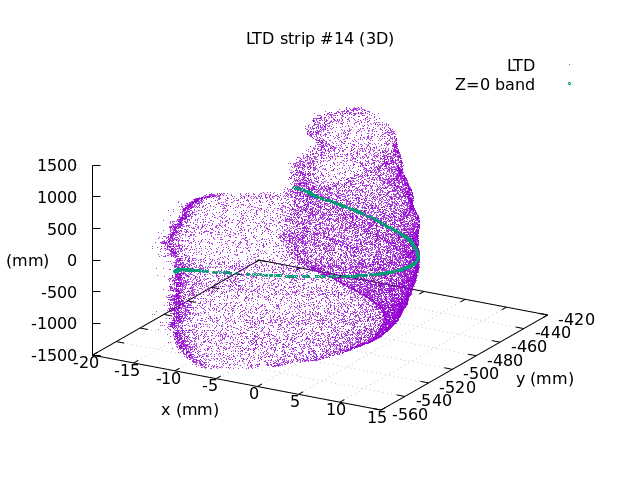
\includegraphics[width=0.45\linewidth]{images/snrs-ltd-strip14-2.png}
      \end{center}
      The deformation changes along the Z-axis :

      \begin{itemize}

      \item suggests a 2D-fit per Z-band in the X-Y plane
        then a combination of all Z-fits to build a full 3D model

      \item suggests an elliptic arc as the basic mathematical model for the 2D-fit

      \end{itemize}

          
   % \end{exampleblock}
  }

  \only<4-5>{

    \begin{block}{Step 2 : build the FSF data \textit{Foil Shaping Fit} (ITEP style foils)}
      
      \begin{itemize}

        \only<4>{
      % \item Described in DocDB \#5425

      \item Extract 101 regularly spaced Z-bands from the calibrated LTD dataset for each ITEP strip ($\Delta{}z\simeq$2.5 cm)

      \item For each Z-band : perform a 2D-fit with an elliptic arc (4 parameters, typically 200 points with Z-band width of 1.5 mm, $NDOF>100$)

        \begin{center}
         \scalebox{0.5}{\input{\pdftextimgpath/snrs-fsf-1.pdftex_t}}
        \end{center}
        }
        \only<5>{
      \item Caveats:
        %\tiny
        \begin{itemize}

        \item we assume a symmetrical shape for the strips 
        \item
         we don't really know the 3D measurement resolution of the laser system $\leadsto$
          use arbitrary value $\sigma_{x,y,z}\simeq$1 mm (possible overestimation of the errors)

        \item laser measurements show some kind of \emph{halo} of 3D-points at the edge
          of all shapes within the detector:

          we have to cut the LTD points near the edges of each source strip to stabilize the fit,
          at the price of ignoring the true position (<1 mm precision) of the foil's bounds

        \item 2D-fits on Z-bands are performed independantly: we do not take into account expected correlations
          of the deformation parameters between two  successive bands
          
        \end{itemize}
        }
        
      \end{itemize}
         
    \end{block}
  }

  \only<6>{
    Fit results for ITEP strip \#32 :
    %%\begin{exampleblock}{Fit results for ITEP strip \#32}
      \begin{center}
        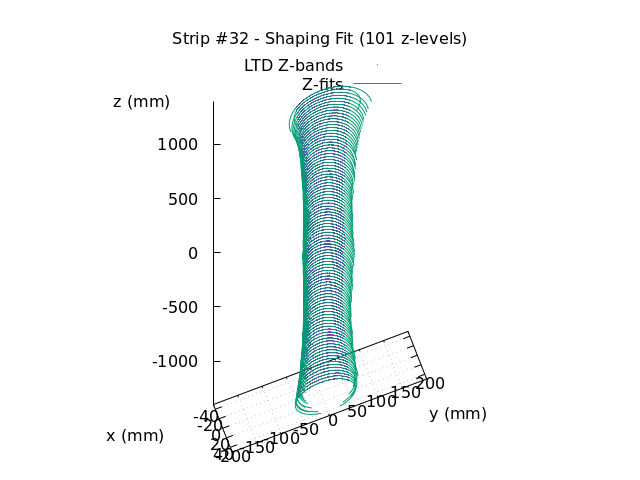
\includegraphics[width=0.75\linewidth]{images/snrs-fsf-strip32-1.png}
      \end{center}
    %%\end{exampleblock}
  }

  \only<7>{
    \vskip -25mm
    %\begin{exampleblock}{
    Fit results for ITEP strip \#32 :
    \vskip 2pt
      %\begin{center}
        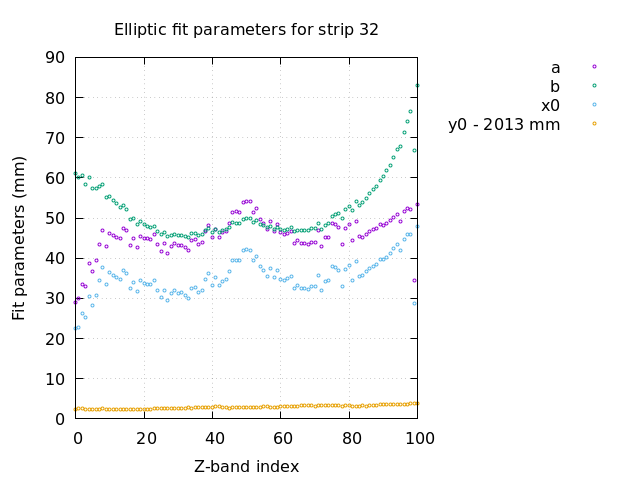
\includegraphics[width=0.65\linewidth]{images/snrs-fsf-strip32-2.png}
        %\end{center}
        
        \noindent Goodness-of-fit: $\chi^2<150$  for $NDOF\simeq200$ $\leadsto$ too good
        (incorrect $\sigma_{x,y,z}$)  
        
      \vskip -15mm
      \hskip 4.65cm $\longleftarrow$ vertical axis of the strip
      \vskip -3.9cm
      \hskip 6.6cm $\left.\right\}$ $a$ and $x_0$ strongly correlated
    %\end{exampleblock}
  }
 
  \only<8>{

    \begin{block}{Step 3 : build a 2D mother mesh}

      \begin{itemize}

      \item Regular sampling of a finite number of vertexes (11) horizontally along each elliptic arcs

        $\leadsto$ multistep numerical quadrature of elliptic integrals
 
      \item Join all horizontal sets of vertexes by vertical edges

        \begin{center}
         \scalebox{0.4}{\input{\pdftextimgpath/snrs-2d-mesh-1.pdftex_t}}
         \scalebox{0.5}{\input{\pdftextimgpath/snrs-2d-mesh-2.pdftex_t}}
        \end{center}

      \item Typically: 11$\times$101 vertexes $\rightarrow$ 1000 quadrangular tiles per foil
    
      \end{itemize}
   
    \end{block}

  }

  \only<9>{
    2D-mesh for ITEP strip \#32 :
    \vskip 2pt
    \hskip -1.5cm
    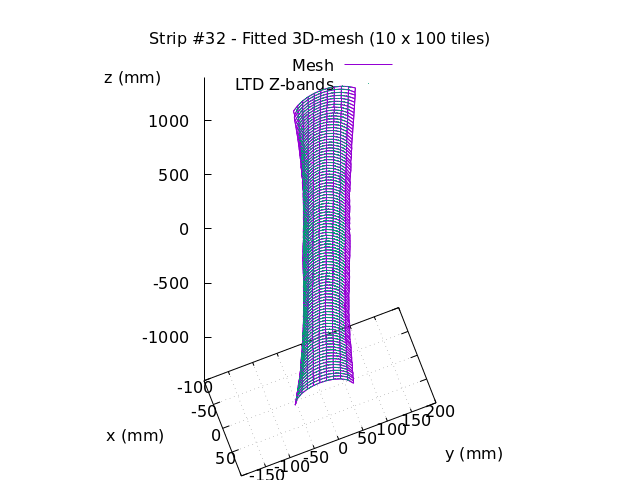
\includegraphics[width=0.75\linewidth]{images/snrs-fsf-strip32-3.png}
    \hskip -1.9cm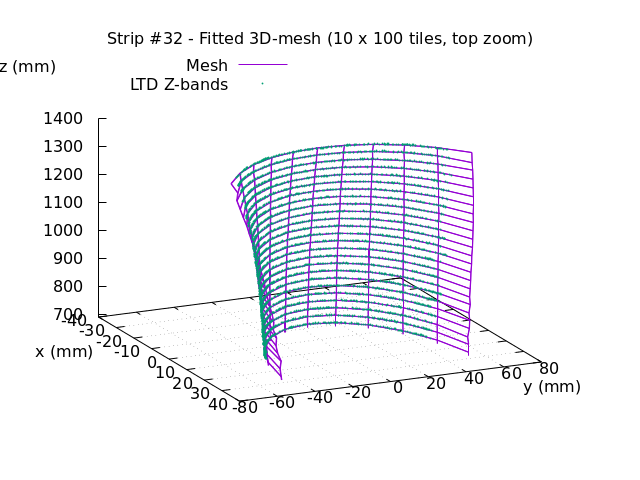
\includegraphics[width=0.55\linewidth]{images/snrs-fsf-strip32-4.png}
    
    %% \noindent Goodness-of-fit: $\chi^2<150$  for $NDOF\simeq200$ $\leadsto$ too good
    %% (incorrect $\sigma_{x,y,z}$)  
    
    %% \vskip -15mm
    %% \hskip 4.65cm $\longleftarrow$ vertical axis of the strip
    %% \vskip -3.9cm
    %% \hskip 6.6cm $\left.\right\}$ $a$ and $x_0$ strongly correlated
  }
 
  \only<10>{

    \begin{block}{Step 3 : build the Bayeux/geomtools 3D geometry model}

      \begin{itemize}

      \item Use the primary 2D-mesh above and give it the proper thickness (100-300 $\mu$m
        depending on the foil) $\leadsto$ 3D-mesh of $\simeq$ 4000 triangular tiles
        for the Se foil:
        \vskip -1cm
        \,
        \begin{center}
         \scalebox{0.4}{\input{\pdftextimgpath/snrs-3d-mesh-1.pdftex_t}}
         \scalebox{0.5}{\input{\pdftextimgpath/snrs-3d-mesh-2.pdftex_t}}
        \end{center}

      \item Generate also \textit{skin} 3D-mesh for
        the two surrounding Mylar foils (12 $\mu$m thickness) 

      \item Result:

        \begin{itemize}

        \item 3 tessellated solids per source strip + absolute placement in the SN coordinate frame

        \item generate data as input for Bayeux/Falaise geometry models

          $\leadsto$ reasonnable amount of memory storage
          
        \end{itemize}
        
      \end{itemize}
   
    \end{block}

  }
 
  \only<11>{
     3D-meshes for ITEP strip \#34 : 2 Mylar films and 1 Selenium strip
    \vskip 2pt
    \begin{center}
    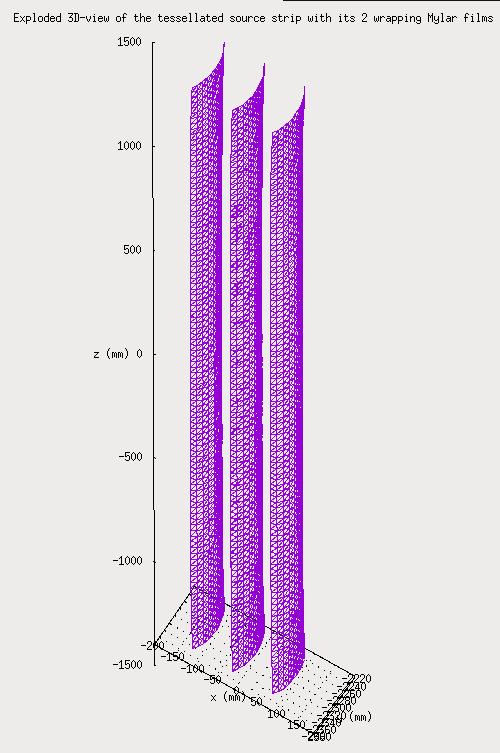
\includegraphics[height=6cm]{images/strip34-source-3d.png}
    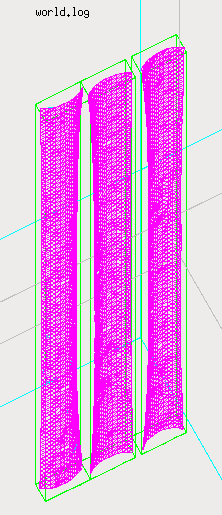
\includegraphics[height=6cm]{images/test-strip-mesh-32-33-34-3d.png}
    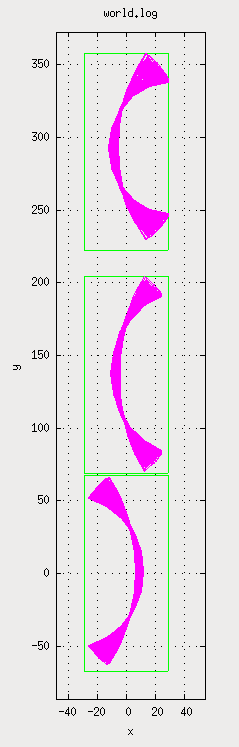
\includegraphics[height=6cm]{images/test-strip-mesh-32-33-34-xy.png}
    \end{center}

    
    \noindent \hskip 4cm ...\, toy integration of foils \#32-34 in Bayeux

  }
 
  \only<12>{
    \begin{block}{Implementation of the \texttt{snrs::mesh\_pad\_model} class}
      \begin{itemize}

      \item New geometry model class (compatible with Bayeux/Falaise)
        
      \item Use the standard configuration system in Bayeux/Falaise:

        Example: source strip \#32
        \tiny
        \vskip 10pt
        \VerbatimInput[frame=single,label={\fbox{Configuration}}]{samples/geo.conf}

        \footnotesize
        
      \item Automated load of pre-calculated 3D-mesh datasets from resource files provided by the package
        
      \end{itemize}
    \end{block}
      
  }
}

%%%%%%%%%%%%%%%%%%%%%%%%%%%%%%%%%%%%%%%%%%%%%%%%%%%%%%%%%%%%%%%
\frame{

  \footnotesize

  \frametitle{The SNRS software package}

  \only<1>{

    \begin{block}{Step 4 : implement vertex generators for ITEP foils realistic model}

      \begin{itemize}
        
      \item Each source strip is modelled through 1000 3D-tiles of supposedly
        equal mass and surface
        (uniform weighting $\leadsto$ fast random sampling)

      \item 3 types of generators needed for different contamination hypotheses:

        \begin{itemize}
        
        \item Outer surfaces (Mylar film): radon or other contaminant deposit

        \item Mylar film bulk: intrinsic radioactive contamination (Bi, Tl\dots)

        \item Selenium source bulk : $^{82}$Se DBD decays + intrinsic radioactive contamination (Bi, Tl\dots)
          
        \end{itemize}

      \item Other possibilities: modelling hot spots on surface or bulk ?

      \end{itemize}

    \end{block}

  }

  \only<2>{


    \begin{block}{First implementation of the \texttt{snrs::mesh\_pad\_vg} class}

      Features:
      \begin{itemize}
        
      \item Surface vertex generator: uniform random sampling on all triangular surface 2D-tiles
        (available)
        
      \item Mylar bulk  vertex generator:
        approximated uniform random sampling inside all triangular bulk tiles
        through normal shifting of vertexes from the surface
        (available)

      \item Selection tools for specific ranges of tiles of set of tiles
        (available)

      \item Source bulk (not available yet)
        
      \end{itemize}
        
    \end{block}

  }

  \only<3>{

    Use the standard configuration system in Bayeux/Falaise:
    \begin{exampleblock}{Example: Surface vertex generator in strip \#32}

      \vskip 10pt
      \VerbatimInput[frame=single,label={\fbox{Configuration}}]{samples/vg.conf}

    \end{exampleblock}
    More features available...
  }

  \only<4>{

    Generation of vertexes on the surfaces (back+front, all tiles, 3D zoomed view) of a source strip:
    \begin{center}
      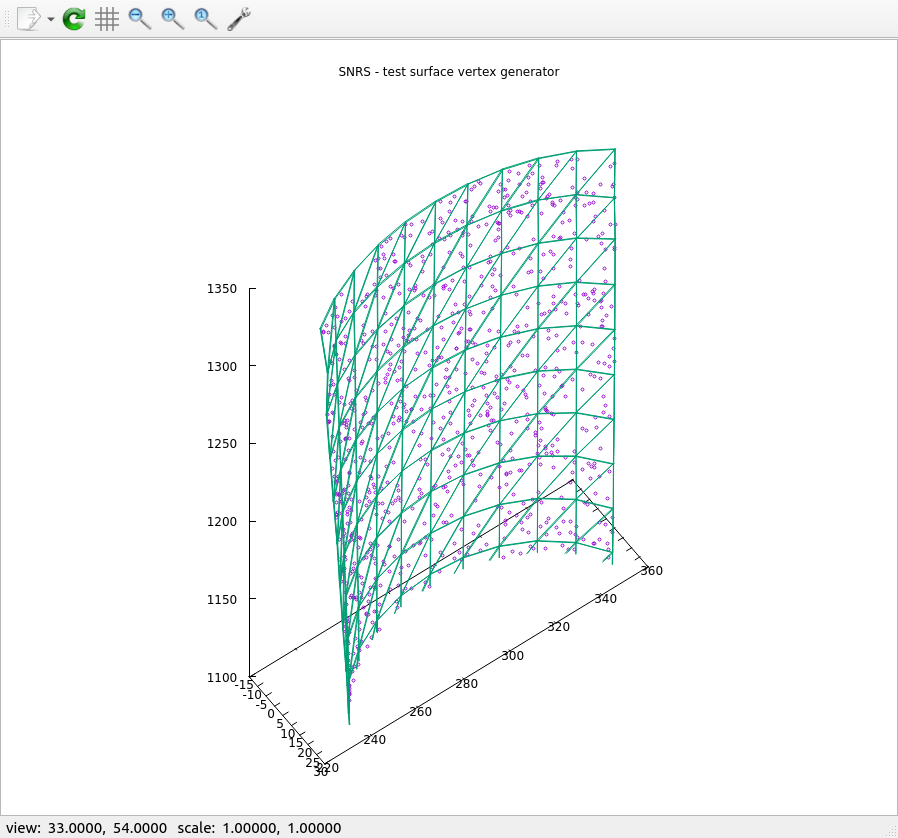
\includegraphics[height=6cm]{images/text_mesh_pad_vg_1.png}
    \end{center}

  }

  \only<5>{

    Selectivity test on back tiles only (Italy) + arbitrary normal shift (exploded zoomed view):
    \begin{center}
      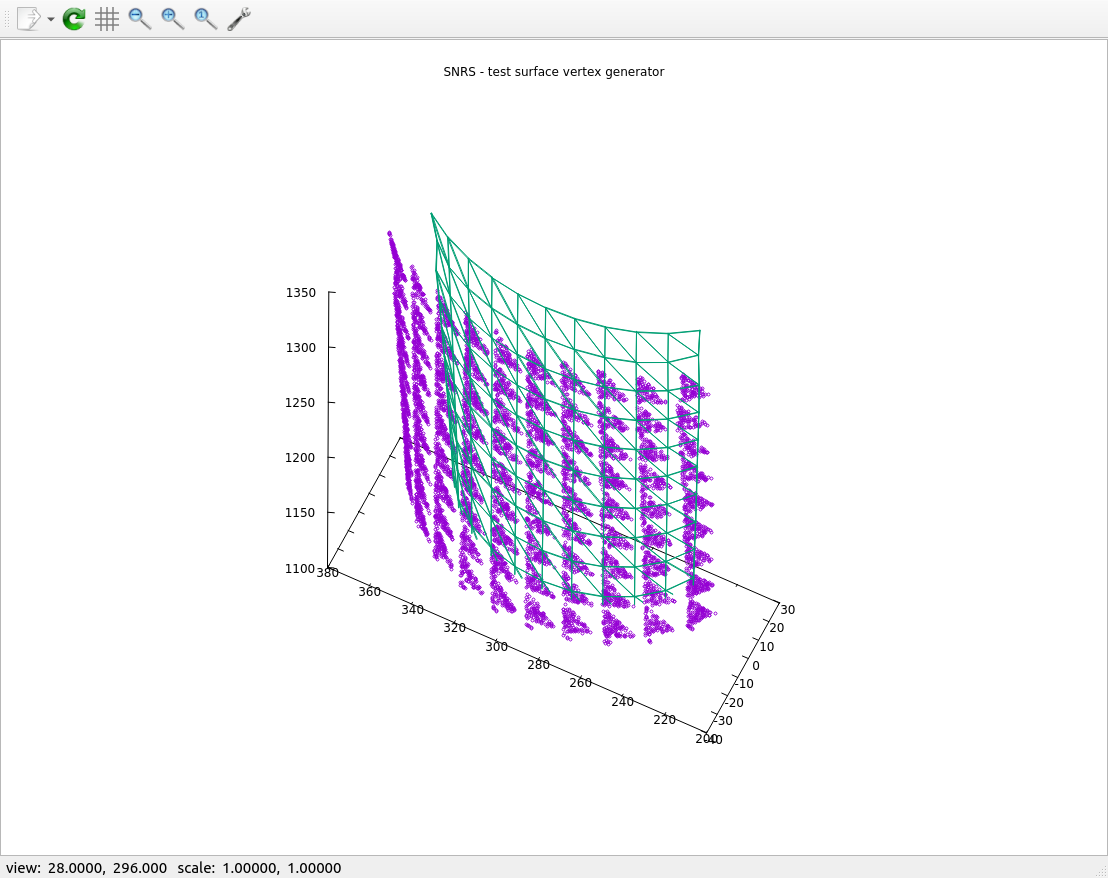
\includegraphics[height=6cm]{images/text_mesh_pad_vg_2.png}
    \end{center}

  }

  \only<6>{

    The Gotham test :
    complex assembly of various vertex generators with specific tile selectors
    on ITEP strips \#32-34 (side Y-Z zoomed viewd zoomed):
    \begin{center}
      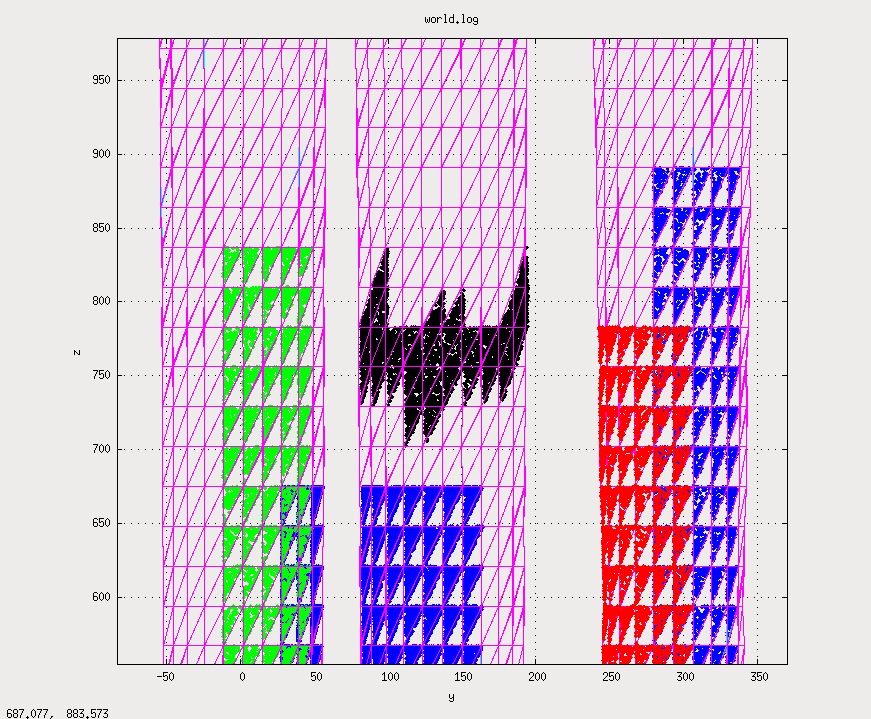
\includegraphics[height=6cm]{images/text_mesh_pad_vg_3.png}
    \end{center}

  }
}

%%%%%%%%%%%%%%%%%%%%%%%%%%%%%%%%%%%%%%%%%%%%%%%%%%%%%%%%%%%%%%%
\frame{

  \footnotesize

  \frametitle{The SNRS software package}

  \begin{block}{Conclusion}
  
  \begin{itemize}
    
  \item Preliminary version of the SNRS package
    \\
    \textcolor{blue}{\texttt{https://github.com/SuperNEMO-DBD/SNRS}}

  \item Not available yet for production but quite mature

  \item All modelling steps 1-4 have been visited/implemented

  \item ITEP source foils 3 to 34 are supported.
    
  \item To be done:
    \begin{itemize}

    %%\item Generalize to all ITEP source foils (currently available : 32, 33, 34)}
      
    \item Implement the \textit{bulk} mode for the new vertex generator engine (for DBD processes\dots)

    \item Bayeux 3.5 release needed
      
    \item Integration in Falaise (link + new geometry/genvtx variants) and tests with \textcolor{blue}{\texttt{flsimulate}}
      
    \item Step 5 : to be implemented, \\
      optimization tools maybe necessary: accelerator(s) for finding intercepts on tiles
      (Bayeux$\oplus$Falaise)
      
    \item What about LAPP 8-pad strips ?
      
    \end{itemize}
    
  \end{itemize}

  \end{block}

}

%%%%%%%%%%%%%%%%%%%%%%%%%%%%%%%%%%%%%%%%%%%%%%%%%%%%%%%%%%%%%%%
\frame{

  \footnotesize

  \frametitle{Update 2021-05-29}


  \only<1-2>{
  \begin{block}{Modelling of all ITEP strips}

    \begin{itemize}

      \only<1-2>{
      \item Modification of the FSF algorithm used to fit LTD datasets and build the 3D mesh
        \only<1>{
          \begin{itemize}
          \item Special processing of the edge of each strip with a preliminary
            manual
            measurement on LTD dataset to define a fiducial region before
            the fit

          \item The \emph{elliptic} fit now uses a 250 $\mu$m sigma on laser positioning and a stabilized fiducual region (less sensitive to our misunderstanding
            of edges position from LTD dataset)

          \item Special Nadaraya-Watson kernel based smoothing procedure applied on fit parameters
            obtained from Z-fit (101 LTD-zbands per strip) to restore some
            expected regularity on the overall shape of the strips  

          \item 3D meshes built assuming symmetrical layout of the deformed strips
            with respect to their vertical axis (because we cannot use a well
            defined left/right edge positioning)

            
          \end{itemize}
        }
      }
      \only<2>{
      \item Strips 3, 8, 9, 14, 15, 20, 21, 22, 23, 24, 25, 26, 27, 28, 31, 32, 33 and 34 have been processed (LTD+FSF algorithms)
      \item Strip 2 is considered as enough flat to be still approximated by a flat box (like in the current Falaise).
      \item Associated 3D mesh models are published in the SNRS package
      }
    \end{itemize}
    

 
  \end{block}
  }
  
 
  \only<3>{

    Preliminary source frame layout before integration in Falaise (YZ view, from Italian side)
    \begin{center}
      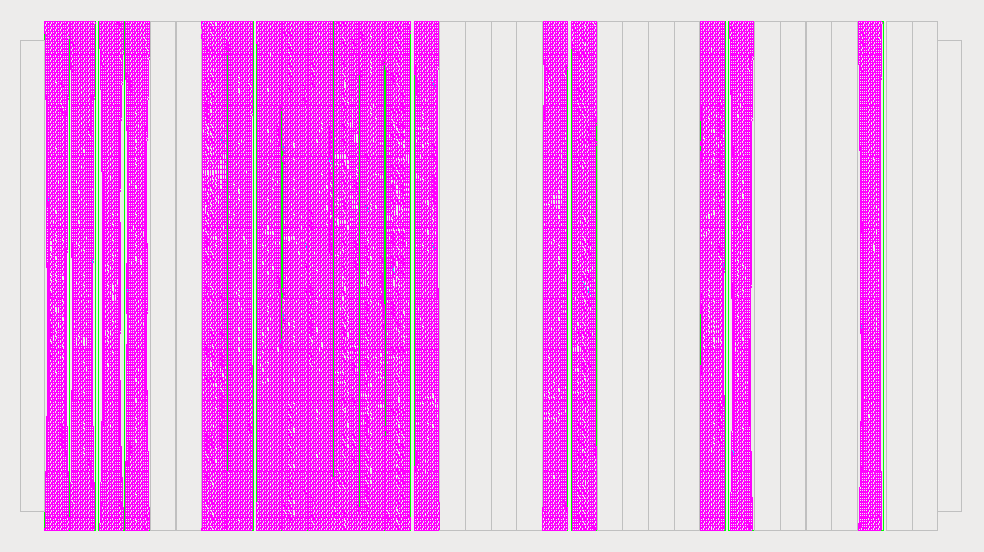
\includegraphics[width=\linewidth]{images/test_realistic_foils_setup_3.png}
    \end{center}

  }
 
  \only<4>{
    \begin{center}
      \textcolor{white}{a\,} \hskip 5pt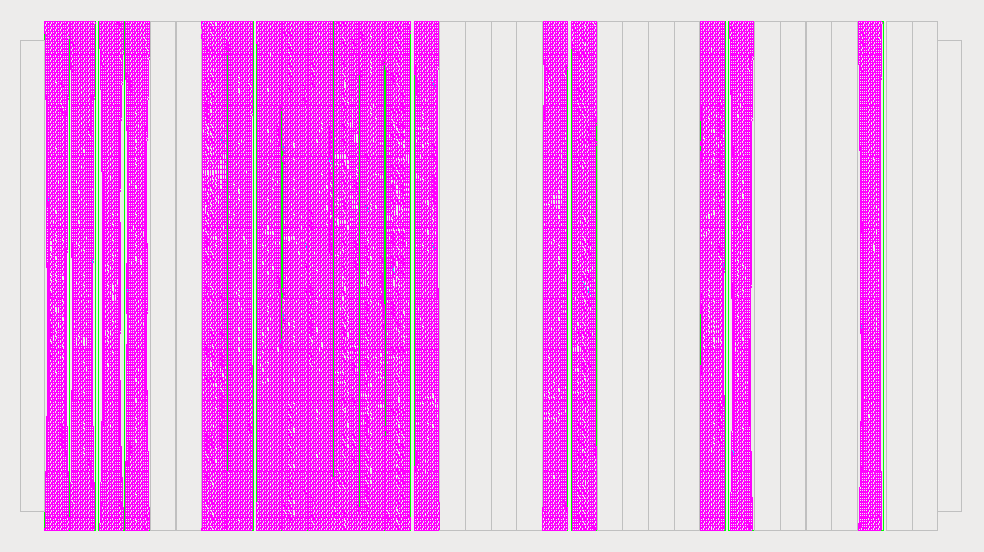
\includegraphics[width=0.47\linewidth]{images/test_realistic_foils_setup_3.png}
      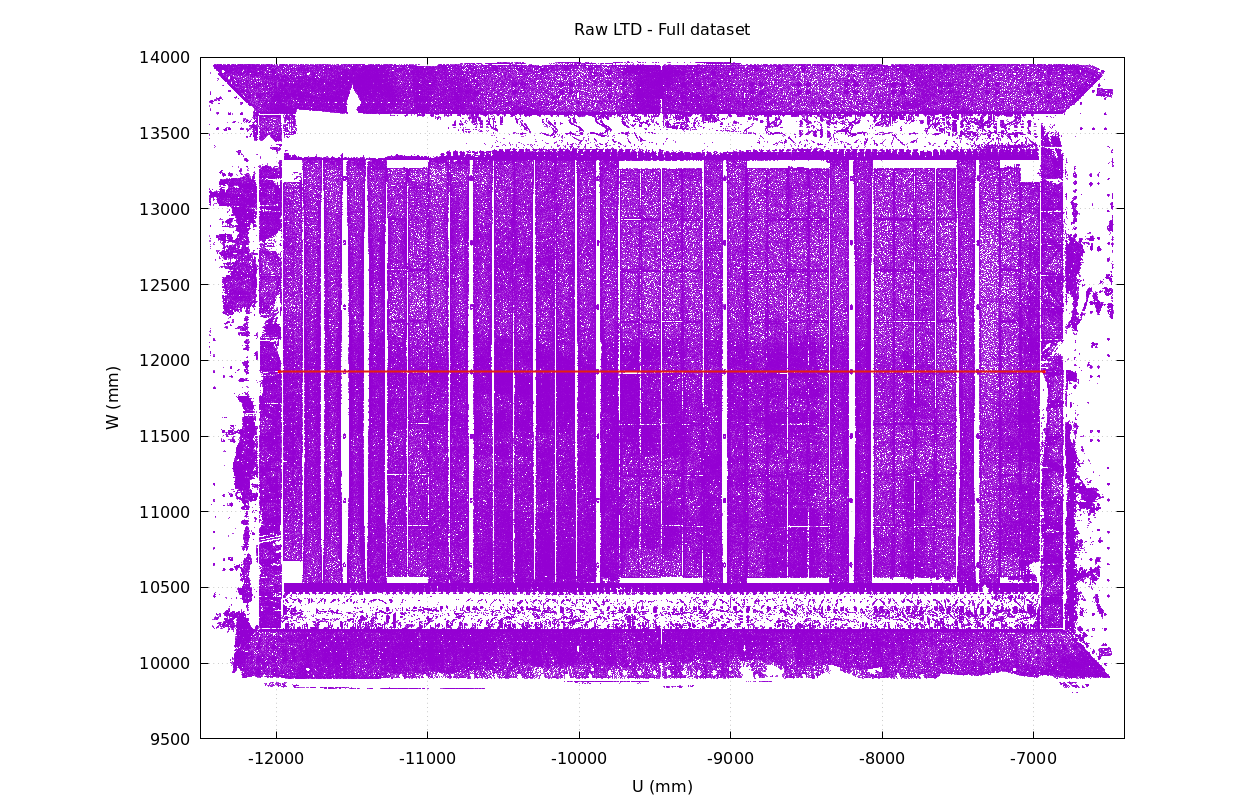
\includegraphics[width=0.75\linewidth]{images/raw_ltd_source_foils_1.png}
    \end{center}

  }

}

\end{document}
